% Revision 10. Concise main text; technical contract retained in appendix.
% Runtime baseline: dec1a40f. Evidence review dated 2026-10-14.
\section{Shared runtime and evaluation harness}
\label{sec:runtime}
\label{sec:measurement}

The runtime provides two of AERead's properties: one kernel executes every
family, and every score is recomputed by code from sealed evidence. The
shared runtime, or \emph{kernel}, executes the case designs in
Section~\ref{sec:task-design}. Families supply the economic rules;
the kernel schedules play and records the evidence used for evaluation
(Figure~\ref{fig:architecture}).

\begin{figure}[htbp]\centering\renewcommand{\thefigure}{4.1}
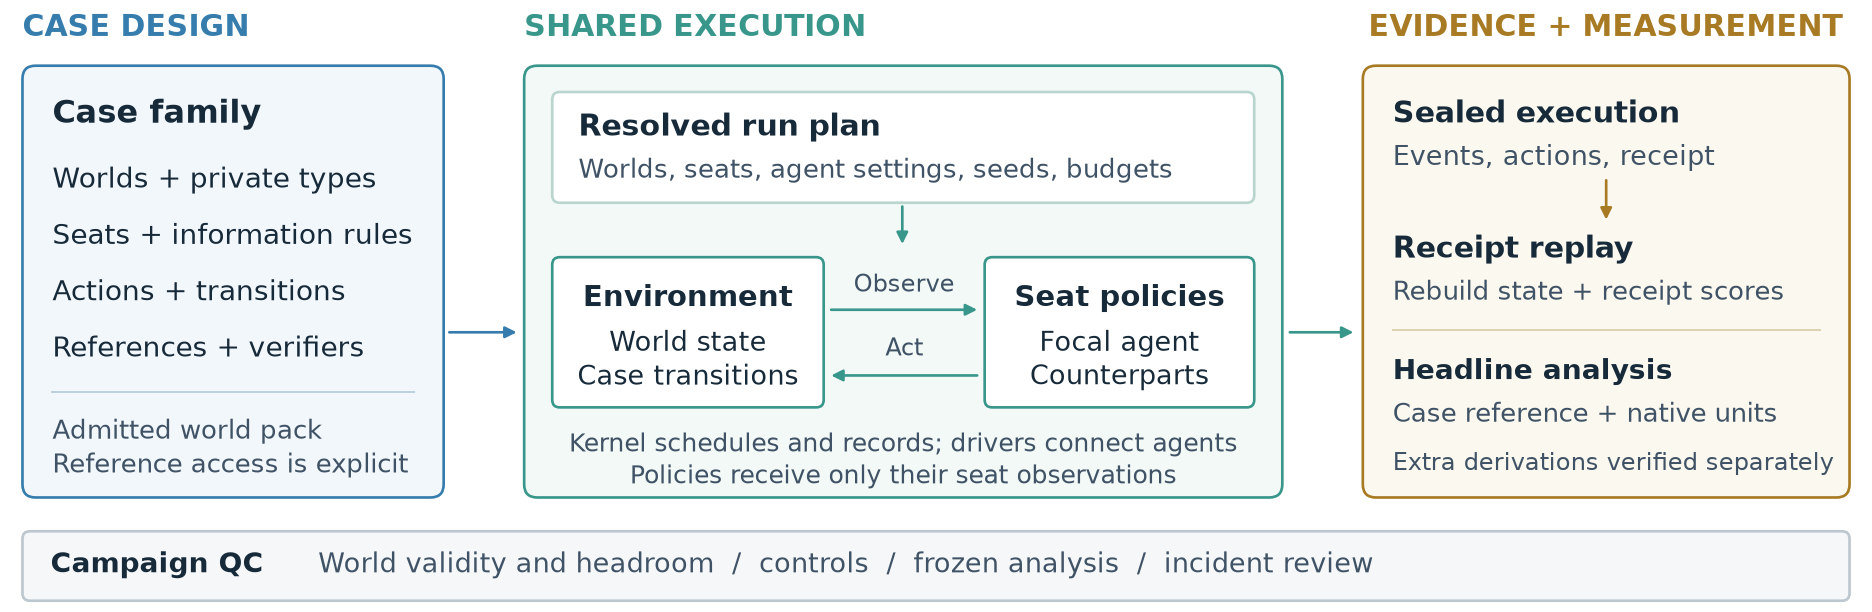
\includegraphics[width=\linewidth]{figures/architecture_overview.png}
\caption{\textbf{AERead architecture.} Families define the economic world and reference; the runtime coordinates seat policies and retains execution evidence. Agents receive only their seat observations, while scoring uses explicitly declared reference access. Replay checks receipt consistency; separate headline derivations require their own verification. Applied coverage and QC verdicts vary by campaign (Appendices F and H).}
\label{fig:architecture}
\end{figure}


\subsection{Verification}
A check compares an action or an outcome with a reference and reports a pass
or fail, a count or an amount. The cases use four kinds of reference. Refund
uses an answer key, which specifies the correct resolution of each claim.
Procurement and the agreement case also check rules, which constrain what
an action may do. Housing, Procurement and the data-center case measure value,
comparing an economic outcome with a policy or a bound. The data-center case also compares named agents
with each other. Results keep their native units, and we report no
cross-family aggregate. A value reference is one of three types: a policy
the evaluated seat could carry out, the best policy given the deciding
seat's information, or a full-information upper bound that the seat need
not be able to reach.

The case-study scores are computed by code. Kernel replay reconstructs
the state and each receipt's score from the recorded actions, without
calling a model. Replay therefore establishes that a score agrees with the
recorded execution. Whether the score measures the intended decision is a
separate question, which the quality-control checks of \qcref{} address.
Housing and Procurement also report headline measures that are computed
outside the receipt and verified separately; Appendix~\ref{app:runtime-cases}
documents how each is computed.

\subsection{Evaluation harness}
Before execution, the kernel hashes a plan that specifies the worlds, seat
assignments, agent configurations, seeds and budgets. During simultaneous
play, it freezes all acting seats' observations before requesting actions
and then applies their joint transition. Calls through its provider and
tool interfaces are logged with typed outcomes. Finalization seals the
evidence and produces a receipt binding the plan, world and scores.

A seat is played in one of three ways. Most models run through AERead's
own harness. Each action is a single call through a pinned provider route.
The call receives the seat's instructions and its current observation, and it
returns one action in the case's schema. It has no tools and no memory beyond
what the observation shows. The harness checks the route against its pin, requests a
seed, and records the specified reasoning setting and output limit.
Gemini 3.8 Flash, GLM 5.3 Flash and GPT-6 Luna in Housing (Gemini and Luna
in Procurement), the Refund models and the TERMS-Bench agents are run this
way.

The two frontier agents, Opus 5.5 and Sol 6.1, run instead through
their vendors' command-line tools, Claude Code and Codex. Each action starts a fresh process
at low reasoning effort, with the same instructions and schema, tools
disabled or refused, and no session carried over. In every comparison reported in
Section~\ref{sec:cases}, both tools ran isolated from the operator's setup.
Claude Code ran in safe mode, with none of the operator's instructions,
memory or skills, in a fresh, neutrally named directory; the account's email
address remained in its context. Codex ran with a fresh home directory that
held only its login, and it listed only its four built-in skills. Before any
world, each tool was probed under the run's exact settings, and a violation
would have stopped the run; none occurred. The agreement case's first
comparison (v1) predates this isolation, and in it Codex listed eight of the
operator's own skills (Table~\ref{tab:cli-controls}). Only the tool's version
and binary are checked, and the tool exposes no seed, temperature or output
limit. Through the harness, the system under evaluation is the model; through a
command-line tool, it is the product, including the tool's own instructions and
internal turns. A comparison across the two paths therefore compares agent
configurations rather than models, and each result names its path.

The third way is a script. Counterparts, references and simple-rule baselines
are scripted, call no model and replay exactly.

A recorded setting does not establish that a provider honoured it.
Appendix~\ref{app:runtime} gives the controls each path applied and the
versions behind each reported panel.
